\section{Related Work}
\subsection{Diffusion Models in Robotics}
Diffusion models, a category of generative models that progressively transform random noise into a data sample, have achieved great success in high-fidelity image generation~\citep{ho2020ddpm, song2020score, rombach2022stable_diffusion,song2020ddim}. Owing to their impressive expressiveness, diffusion models have recently been applied in robotics, including in fields such as reinforcement learning~\citep{wang2022diffusion_QL,ajay2022conditional_generative_modeling}, imitation learning~\citep{chi2023diffusion_policy, pearce2023imitating_diffusion, reuss2023goal,xian2023chaineddiffuser,sridhar2024memoryconsistent,prasad2024consistency}, reward learning~\citep{Huang2023DiffusionReward,nuti2023extracting}, grasping~\citep{wu2023graspGF,urain2023se3,simeonov2023shelving}, and motion planning~\citep{saha2023edmp,janner2022diffusion_planning}. In this work, we focus on representing visuomotor policies as conditional diffusion models, referred to as \textit{diffusion policies}, following the framework established in \citep{chi2023diffusion_policy,pearce2023imitating_diffusion}. Unlike prior methods that primarily focus on images and states as conditions, we pioneer in incorporating 3D conditioning into diffusion policies.

\subsection{Visual Imitation Learning}
\label{section: visual imitation learning}
Imitation learning offers an efficient way for robots to acquire human-like skills, typically relying on extensive observation-action pairs from expert demonstrations. Given the challenges in accurately estimating object states in the real world, visual observations such as images have emerged as a practical alternative. While 2D image-based policies~\citep{pari2021VINN,florence2022ibc,chi2023diffusion_policy,mandlekar2021robomimic,haldar2023fish, shafiullah2022bet, wang2023mimicplay,ha2023scaling} have predominated the field, the significance of 3D is increasingly recognized~\citep{shridhar2023peract,ze2023gnfactor,Ze2022rl3d,goyal2023rvt,gervet2023act3d,3d_diffuser_actor,wang2024dexcap}.


\revise{Recent 3D-based policies, including PerAct~\citep{shridhar2023peract}, GNFactor~\citep{ze2023gnfactor}, RVT~\citep{goyal2023rvt}, ACT3D~\citep{gervet2023act3d}, and NeRFuser~\citep{yan2024nerfuser}, have demonstrated notable advancements in low-dimensional control tasks. However, these works face two primary challenges: (1) \textbf{Impractical setting.} These methods convert the imitation learning problem into a prediction-and-planning paradigm using keyframe pose extraction. While effective, this formulation is less suitable for high-dimensional control tasks. (2) \textbf{Slow inference.} The intricate architectures of these methods result in slow inference speeds. For instance, PerAct~\citep{shridhar2023peract} runs at an inference speed of 2.23 FPS, making it hard to address tasks that require dense commands, such as highly dynamic environments. Another closely related work 3D Diffuser Actor~\citep{3d_diffuser_actor} runs at 1.67 FPS mainly due to the usage of attention to language tokens and the difference in the task setting\footnote{The inference speed depends on a number of factors, such as the number of camera views used, the input observation size in pixels, the number of diffusion timesteps and the temporal horizon of prediction. Since the two papers tested on different setups, the authors of 3D Diffuser Actor~\citep{3d_diffuser_actor} used DP3’s code to set it up on CALVIN, a multi-task language-conditioned setup. They equipped DP3 with attention to language tokens, identical to their model for fair comparison. They used two cameras to unproject and obtain a point cloud. They ran both DP3 and 3D Diffuser Actor on the same NVIDIA 2080 Ti GPU. Inference for 3D Diffuser Actor takes 600ms and predicts 6 action steps. Inference for DP3 takes 581ms and predicts 4 action steps. As a result, the control frequency of 3D Diffuser Actor on CALVIN is higher than DP3's.}.
Compared to this line of works, we endeavor to develop a universal and fast 3D policy capable of tackling a broader spectrum of robotic tasks, encompassing both high-dimensional and low-dimensional control tasks.}

\begin{figure*}[t]
    \centering    
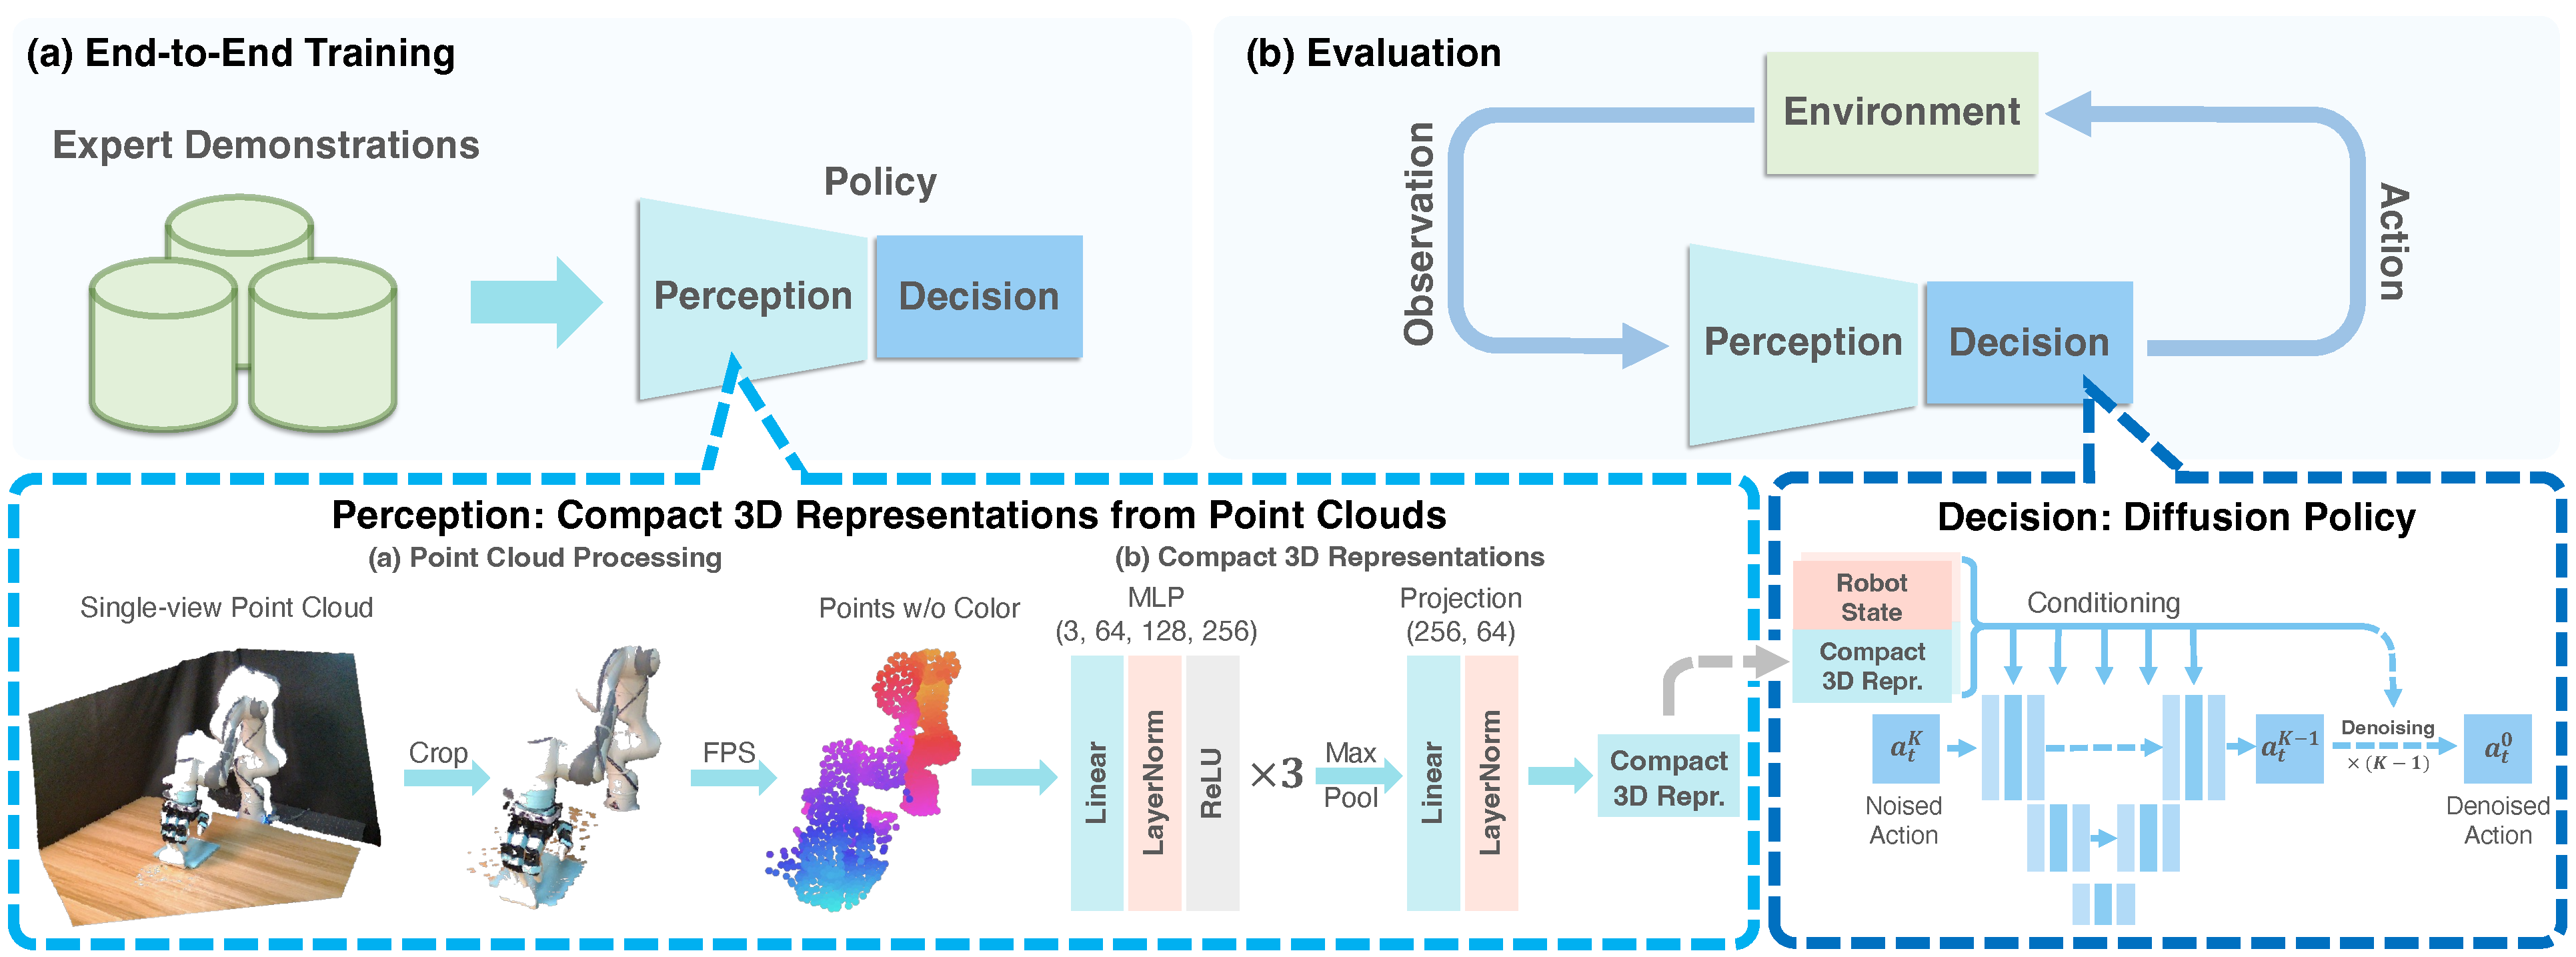
\includegraphics[width=1.0\textwidth]{figures/method_v3.pdf}
    \caption{\textbf{Overview of 3D Diffusion Policy (DP3).} \textbf{Above:} In the training phase, DP3 simultaneously trains its perception module and decision-making process in an end-to-end manner using expert demonstrations. During evaluation, DP3 determines actions based on visual observations from the environment.
\textbf{Below:} DP3 perceives its environment through single-view point clouds. These are transformed into compact 3D representations by a lightweight MLP encoder. Subsequently, DP3 generates actions conditioning on these 3D representations and the robot's states, using a diffusion-based backbone.}
    \label{fig:method}
    \vspace{-0.2in}
\end{figure*}


\subsection{Learning Dexterous Skills} 
Achieving human-like manipulation skills in robots has been a longstanding objective pursued by robotics researchers. Reinforcement learning has been a key tool in this endeavor, enabling robots with dexterous hands to master a variety of tasks, such as pouring water~\citep{qin2022dexmv,ze2023hindex}, opening doors~\citep{rajeswaran2017dapg,hansen2023modem,chen2022bidexhands}, rotating objects~\citep{qi2023hora,yin2023rotating,yuan2023robot_synthethesia,qi2023general_hora}, reorienting objects~\citep{handa2023dextreme,chen2023visual_dex,chen2022system}, spinning pens~\citep{ma2023eureka}, grasping tools~\citep{agarwal2023functional}, executing handovers~\citep{zhang2023flexible_handover,huang2023dynamic_handover}, and building Legos~\citep{chen2023sequential}. Imitation learning offers another pathway, with approaches like DIME~\citep{arunachalam2023dime} and DexMV~\citep{qin2022dexmv} translating human hand movements into robotic actions through retargeting and enabling learning from human videos. Our work, however, diverges from these specific design-centric methods. We demonstrate that enabling the acquisition of these complex skills with minimal demonstrations could be achieved by improving the imitation learning algorithm itself. 
